% Autor: Elias Welt
\section{Authentifizierungsflow: Registrierung und E-Mail-Bestätigung}

Der Authentifizierungsprozess von EduShelf umfasst drei aufeinander aufbauende Schritte: die Registrierung eines neuen Benutzerkontos, die Verifikation der E-Mail-Adresse sowie den eigentlichen Login. Diese Abfolge stellt sicher, dass nur Nutzer mit einer verifizierten Identität Zugang zur Plattform erhalten.

\newpage
\subsection{Registrierung (Register.jsx)}
\begin{figure}[h]
    \centering
    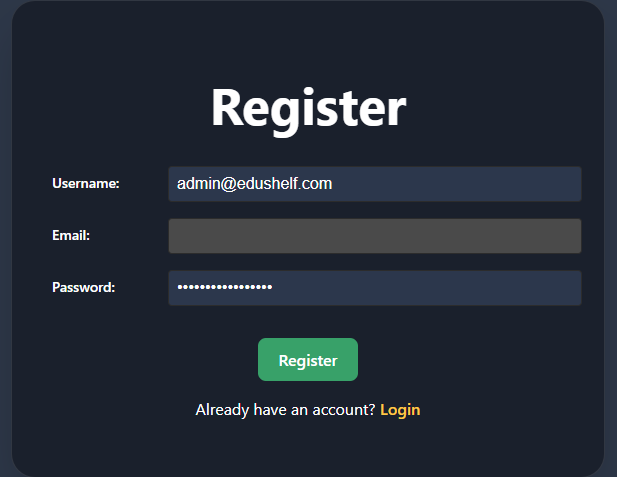
\includegraphics[width=0.82\textwidth]{img/register-dark-mode}
    \caption{Registrierungsformular von EduShelf im Dark-Mode}
    \label{fig:register}
\end{figure}

Die Komponente \texttt{Register.jsx} realisiert ein zweistufiges Validierungskonzept. Zunächst wird die Benutzereingabe vollständig clientseitig geprüft, bevor eine Anfrage an den Server gesendet wird. Dies reduziert unnötige Netzwerkanfragen und gibt dem Nutzer sofortiges Feedback.

\subsubsection{Clientseitige Validierung}

Die Validierungsfunktion überprüft alle Felder nach klar definierten Regeln:

\begin{lstlisting}[language=JavaScript, caption={Clientseitige Eingabevalidierung im Registrierungsformular}]
const validate = () => {
  const newErrors = {};
  if (!username || username.length < 3 || username.length > 20) {
    newErrors.username = 'Username must be between 3 and 20 characters.';
  }
  if (!email || !/\S+@\S+\.\S+/.test(email)) {
    newErrors.email = 'A valid email address is required.';
  }
  if (!password || password.length < 6) {
    newErrors.password = 'Password must be at least 6 characters long.';
  }
  setErrors(newErrors);
  return newErrors;
};
\end{lstlisting}

Diese Methode setzt auf reguläre Ausdrücke zur E-Mail-Validierung und explizite Längenprüfungen für Benutzername und Passwort. Nur wenn \texttt{validate()} ein leeres Fehlerobjekt zurückgibt (d.\,h. \texttt{Object.keys(validationErrors).length === 0}), wird die Backend-Anfrage ausgelöst.

\subsubsection{Serverseitige Fehlerverarbeitung}

Serverseitige Fehler (z.\,B. ein bereits verwendeter Benutzername) werden strukturiert verarbeitet. Das Backend sendet ein Fehlerobjekt mit feldspezifischen Nachrichten zurück, welches das Frontend auflöst und den entsprechenden Feldern zuordnet:

\begin{lstlisting}[language=JavaScript, caption={Verarbeitung von Backend-Validierungsfehlern}]
if (error.response?.data?.errors) {
  const backendErrors = {};
  for (const key in error.response.data.errors) {
    // Schluessel mit Kleinbuchstaben normalisieren (z.B. "Username" -> "username")
    const formattedKey = key.charAt(0).toLowerCase() + key.slice(1);
    backendErrors[formattedKey] = error.response.data.errors[key].join(' ');
  }
  setErrors(backendErrors);
}
\end{lstlisting}

Diese Normalisierung des Schlüssels (erster Buchstabe zu Kleinbuchstaben) ist notwendig, da das Backend C\#-Konventionen mit großem Anfangsbuchstaben verwendet (\texttt{Username}), während React-State-Schlüssel der JavaScript-Konvention (camelCase) folgen.

\subsection{Login-Prozess (Login.jsx)}

\begin{figure}[h]
    \centering
    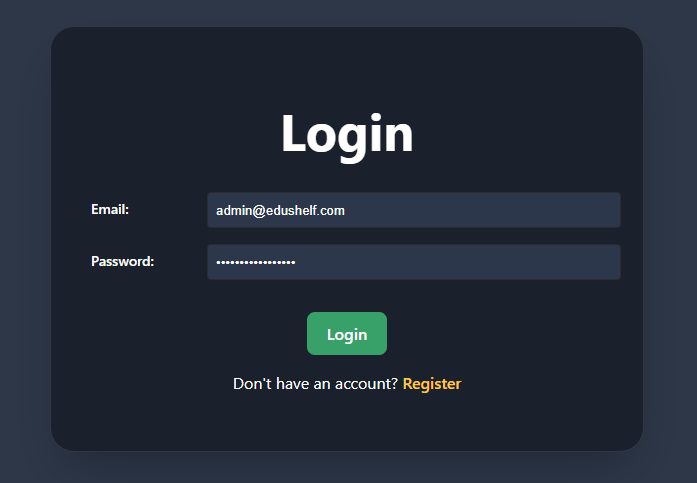
\includegraphics[width=0.82\textwidth]{img/login-dark-mode}
    \caption{Login-Ansicht von EduShelf im Dark-Mode}
    \label{fig:login}
\end{figure}

Der Login-Prozess ist bewusst zweigliedrig gestaltet: Nach dem erfolgreichen POST-Request an \texttt{/Users/login} wird unmittelbar ein zweiter Aufruf an \texttt{/Users/\{id\}/roles} durchgeführt. Die Rollenzuweisung ist für die Steuerung der Navigation essenziell -- nur Nutzer mit der Rolle \textit{Admin} sehen den Menüpunkt zum Administrationsbereich.

Das zusammengesetzte Benutzerobjekt (Nutzerdaten + Rollen) wird im \texttt{localStorage} abgelegt, um den Anmeldestatus über Browser-Refreshes hinweg zu erhalten. Diese Persistierung gilt ausschließlich der UI-Zustandsverwaltung; die tatsächliche Sitzungsauthentifizierung erfolgt serverseitig über ein HttpOnly-Cookie.

\subsection{E-Mail-Bestätigung}

Nach der Registrierung erhält der Nutzer eine Bestätigungs-E-Mail. Der enthaltene Link führt zur Komponente \texttt{VerifyEmail.jsx}, welche den Token aus der URL extrahiert und an den Backend-Endpunkt zur Verifikation übermittelt. Da das Backend den Link selbst generiert, enthält das Frontend lediglich die Anzeigelogik für die Erfolgs- bzw. Fehlermeldung -- eine klare Umsetzung des Single-Responsibility-Prinzips.
